\chapter{การประเมินผล}
\label{Ch:Evaluation}

การประเมินผลของระบบ {\italicfont PyGreenSense} มุ่งเน้นการตรวจสอบทั้งในระดับไลบรารีสำหรับตรวจจับ {\italicfont Green Code Smell} และในระดับส่วนขยาย {\italicfont Visual Studio Code (VS Code Extension)} เพื่อประเมินความถูกต้อง ความน่าเชื่อถือ และความเหมาะสมในการใช้งานจริงของระบบ โดยแนวทางการประเมินแบ่งออกเป็น 2 ส่วนหลัก ได้แก่ (1) การประเมินผลไลบรารี และ (2) การประเมินผลส่วนขยาย VS Code

นอกจากนี้ แนวทางการประเมินยังพิจารณาใน 3 มิติสำคัญ ได้แก่ การเปรียบเทียบผลก่อนและหลังใช้งานในด้านพลังงาน การเปรียบเทียบผลกับเครื่องมือที่ใกล้เคียง และการวัดผลจากการใช้งานจริงของผู้ใช้

% -----------------------------------------------------

\section{การประเมินผลไลบรารี}

การประเมินผลในระดับไลบรารีมีวัตถุประสงค์เพื่อพิสูจน์ว่าระบบตรวจจับ {\italicfont Green Code Smell} ที่พัฒนาขึ้นสามารถทำงานได้อย่างมีประสิทธิภาพในสถานการณ์ที่ใกล้เคียงกับการใช้งานจริง โดยเน้นการเปรียบเทียบความสามารถในการตรวจจับกับเครื่องมือที่เป็นที่รู้จักในอุตสาหกรรม เพื่อสร้างความเชื่อมั่นต่อผลการวิเคราะห์ของระบบ

\subsection{ชุดข้อมูลและเครื่องมือที่ใช้ในการทดสอบ}

ในการประเมินผลครั้งนี้ ใช้ซอร์สโค้ดภาษา Python ขนาดประมาณ 5{,}000 บรรทัด (LOC) เพื่อจำลองลักษณะของโปรเจกต์ที่มีความซับซ้อนในระดับการใช้งานจริง โดยเลือกเครื่องมืออ้างอิงสำหรับการเปรียบเทียบดังนี้

\begin{itemize}
    \item {\boldfont Vulture} สำหรับการตรวจจับ {\italicfont Dead Code}
    \item {\boldfont PyExamine} สำหรับการตรวจจับ {\italicfont Long Method} และ {\italicfont Large Class (God Class)}
    \item {\boldfont Smell-detector-python} สำหรับการตรวจจับ {\italicfont Long Method}
\end{itemize}

แนวทางดังกล่าวช่วยให้สามารถเปรียบเทียบความสามารถของ {\boldfont PyGreenSense} กับเครื่องมือเฉพาะทางที่มีการใช้งานอยู่แล้ว และช่วยยืนยันว่า {\italicfont logic} การตรวจจับของระบบมีความสอดคล้องกับแนวทางมาตรฐานในงานวิเคราะห์โค้ด

\subsection{ผลการเปรียบเทียบการตรวจจับ Code Smell}

การทดสอบเชิงเปรียบเทียบ ({\boldfont Benchmarking}) ถูกใช้เพื่อประเมินว่า {\boldfont PyGreenSense} สามารถตรวจจับ {\italicfont Green Code Smell} แต่ละประเภทได้ครอบคลุมและมีความสอดคล้องกับเครื่องมืออ้างอิงเพียงใด โดยการประเมินในส่วนนี้ครอบคลุมอย่างน้อยปัญหาสำคัญ เช่น {\boldfont Dead Code}, {\boldfont Long Method} และ {\boldfont God Class} ซึ่งเป็น {\italicfont code smell} ที่มีความสัมพันธ์กับคุณภาพของโค้ดและอาจส่งผลต่อพลังงานของซอฟต์แวร์ได้ \cite{verdecchia2018energy}

ผลการประเมินในมิตินี้พิจารณาจากประเด็นสำคัญดังต่อไปนี้

\begin{itemize}
    \item จำนวนปัญหาที่ระบบตรวจพบในแต่ละประเภท
    \item ความสอดคล้องของผลลัพธ์กับเครื่องมืออ้างอิง
    \item กรณีที่ระบบตรวจพบเพิ่มเติมจากเครื่องมืออ้างอิง หรือกรณีที่มีความแตกต่างในการตีความ
    \item ความสามารถในการตรวจจับ {\italicfont smell} ที่สัมพันธ์กับบริบทด้าน {\italicfont Green Software Engineering}
\end{itemize}

\begin{table}[H]
    \centering
    \begin{tabularx}{\textwidth}{>{\raggedright\arraybackslash}p{3cm} >{\raggedright\arraybackslash}p{4cm} X}
        \toprule
        {\boldfont ประเภท Code Smell} & {\boldfont ผลการเปรียบเทียบ (Benchmarking)} & {\boldfont หมายเหตุ} \\
        \midrule
        Dead Code
        & ตรงกันกับเครื่องมือ Vulture
        & ตรวจพบฟังก์ชันและตัวแปรที่ไม่ได้ใช้งานได้อย่างแม่นยำ \\
        Long Method
        & ตรงกันกับ PyExamine และ smell-detector-python
        & มีการคำนวณจำนวนบรรทัดในฟังก์ชันที่สอดคล้องกัน \\
        God Class
        & ตรงกันกับ PyExamine
        & ตรวจจับคลาสที่มีขนาดใหญ่เกินไป ({\italicfont Large Class}) ได้อย่างถูกต้อง \\
        Duplicated Code
        & มีความแตกต่างในด้านขอบเขตการตรวจจับ
        & เครื่องมืออื่นมักตรวจแบบข้ามไฟล์ ({\italicfont Cross-file}) แต่ในเวอร์ชันปัจจุบันของ {\italicfont PyGreenSense} เน้นการตรวจภายในไฟล์เดียวกัน ({\italicfont Single-file}) \\
        Mutable Default Argument
        & ตรวจสอบด้วยตนเอง ({\italicfont Manual})
        & เนื่องจากไม่พบเครื่องมืออัตโนมัติที่รองรับกฎนี้ จึงใช้วิธีนับบรรทัดที่มีการประกาศ \texttt{list}/\texttt{dict} ในพารามิเตอร์ฟังก์ชัน \\
        \bottomrule
    \end{tabularx}
\captionsetup{justification=centering, name=ตาราง}
\caption{ผลการเปรียบเทียบการตรวจจับ Code Smell}
\label{tab:benchmark-smells}
\end{table}

\subsection{ตัวอย่างผลการเปรียบเทียบกับเครื่องมืออ้างอิง}

นอกจากผลในตาราง \ref{tab:benchmark-smells} แล้ว ผู้จัดทำยังรวบรวมตัวอย่างผลลัพธ์จากการรันจริงเพื่อเปรียบเทียบรูปแบบการรายงานของ {\italicfont PyGreenSense} กับเครื่องมืออ้างอิงในแต่ละกรณีศึกษา ดังรูป \ref{fig:ch5_deadcode_benchmark} ถึงรูป \ref{fig:ch5_godclass_benchmark}

\begin{figure}[H]
    \centering
    \begin{subfigure}[t]{0.48\textwidth}
        \centering
        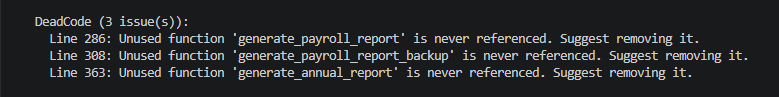
\includegraphics[width=\textwidth]{figures/chap5/benchmark_deadcode_pygreensense.png}
        \captionsetup{name=รูป}
        \caption{ผลจาก PyGreenSense}
    \end{subfigure}
\hfill
\begin{subfigure}[t]{0.48\textwidth}
    \centering
    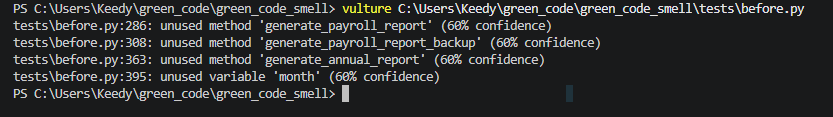
\includegraphics[width=\textwidth]{figures/chap5/benchmark_deadcode_vulture.png}
    \captionsetup{name=รูป}
    \caption{ผลจาก Vulture}
\end{subfigure}
\captionsetup{name=รูป}
\caption{ตัวอย่างการเปรียบเทียบการตรวจจับ Dead Code ระหว่าง PyGreenSense และ Vulture}
\label{fig:ch5_deadcode_benchmark}
\end{figure}

\begin{figure}[H]
    \centering
    \begin{subfigure}[t]{0.48\textwidth}
        \centering
        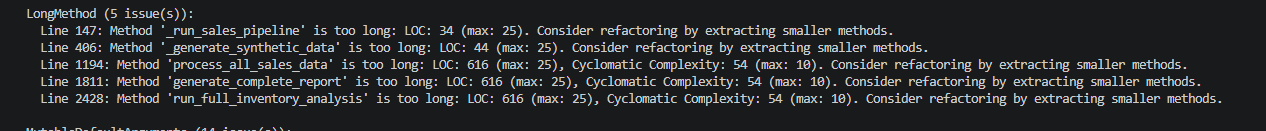
\includegraphics[width=\textwidth]{figures/chap5/benchmark_longmethod_pygreensense.png}
        \captionsetup{name=รูป}
        \caption{ผลจาก PyGreenSense}
    \end{subfigure}
\hfill
\begin{subfigure}[t]{0.48\textwidth}
    \centering
    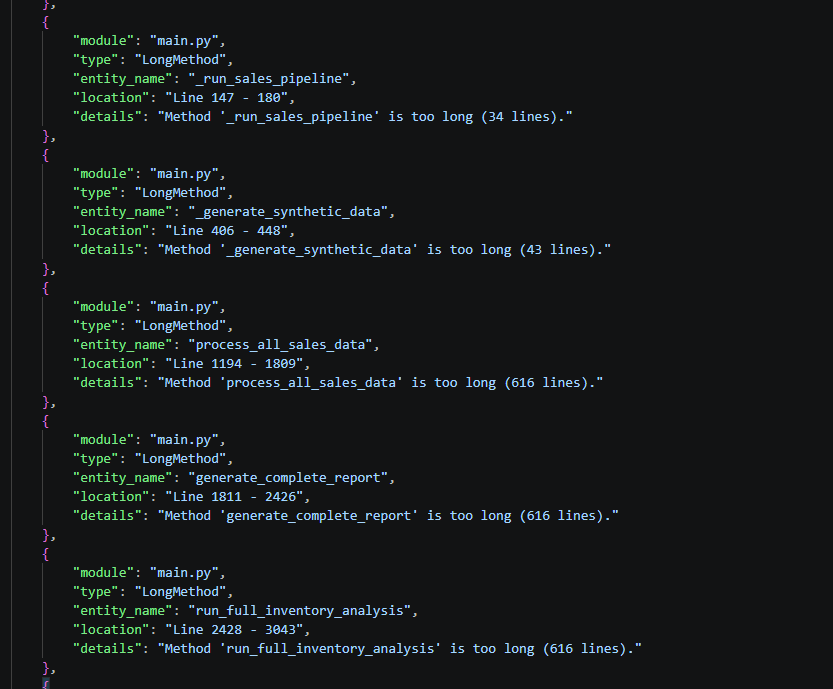
\includegraphics[width=\textwidth]{figures/chap5/benchmark_longmethod_smell_detector.png}
    \captionsetup{name=รูป}
    \caption{ผลจาก Smell-detector-python}
\end{subfigure}
\captionsetup{name=รูป}
\caption{ตัวอย่างการเปรียบเทียบการตรวจจับ Long Method ระหว่าง PyGreenSense และ Smell-detector-python}
\label{fig:ch5_longmethod_benchmark}
\end{figure}

\begin{figure}[H]
    \centering
    \begin{subfigure}[t]{0.76\textwidth}
        \centering
        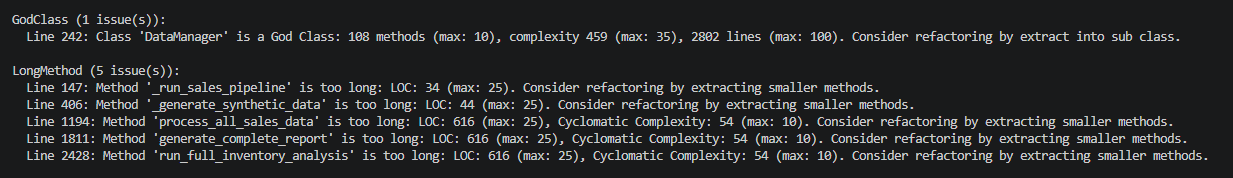
\includegraphics[width=\textwidth]{figures/chap5/benchmark_godclass_pygreensense.png}
        \captionsetup{name=รูป}
        \caption{ผลจาก PyGreenSense}
    \end{subfigure}
\hfill
\begin{subfigure}[t]{0.18\textwidth}
    \centering
    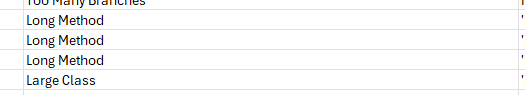
\includegraphics[width=\textwidth]{figures/chap5/benchmark_godclass_pyexamine.png}
    \captionsetup{name=รูป}
    \caption{ผลจาก PyExamine}
\end{subfigure}
\captionsetup{name=รูป}
\caption{ตัวอย่างการเปรียบเทียบการตรวจจับ God Class ระหว่าง PyGreenSense และ PyExamine}
\label{fig:ch5_godclass_benchmark}
\end{figure}

จากรูปข้างต้นจะเห็นว่า {\italicfont PyGreenSense} สามารถรายงานปัญหาในรูปแบบที่อ่านง่ายและเชื่อมโยงกับรายละเอียดเชิงโครงสร้างของโค้ดได้ชัดเจน ขณะที่เครื่องมืออ้างอิงบางตัวอาจรายงานผลในรูปแบบข้อความหรือไฟล์ข้อมูลที่ต่างกัน เช่น {\italicfont PyExamine} ที่แสดงผลเชิงตาราง/CSV และ {\italicfont Smell-detector-python} ที่แสดงผลเชิง JSON หรือ log ทั้งนี้จำนวน smell ที่ตรวจพบอาจไม่เท่ากันทุกเครื่องมือเนื่องจากแต่ละระบบใช้ threshold และตรรกะการตีความปัญหาที่ต่างกัน

\subsection{การวิเคราะห์ผลในระดับไลบรารี}

ในมิติของไลบรารี จุดเด่นของ {\italicfont PyGreenSense} ไม่ได้จำกัดอยู่เพียงการตรวจจับ {\italicfont code smell} แบบทั่วไปเท่านั้น แต่ยังมุ่งเชื่อมโยงผลการตรวจจับเข้ากับแนวคิดด้านพลังงานและความยั่งยืนของซอฟต์แวร์ ซึ่งสอดคล้องกับกรอบแนวคิดของ {\italicfont Green Software Engineering} และ {\italicfont Green Code Smells} \cite{leGoaer2024tactics,legoaer2023ecocode} ผลลัพธ์ที่ได้จากไลบรารีจึงมีความเหมาะสมสำหรับใช้เป็นฐานข้อมูลในการวิเคราะห์ต่อยอดด้านคาร์บอน พลังงาน และตัวชี้วัดเชิงฟังก์ชันในขั้นถัดไป

% -----------------------------------------------------

\section{การประเมินผลจากชุดโค้ดทดสอบ}

การประเมินผลจากชุดโค้ดทดสอบมีวัตถุประสงค์เพื่อพิจารณาว่า การตรวจจับและการปรับปรุงโค้ดตามแนวทางของ {\italicfont PyGreenSense} สามารถสะท้อนผลลัพธ์ในเชิงโครงสร้างของโค้ด มาตรวัดเชิงฟังก์ชัน และค่าพลังงานหรือคาร์บอนได้อย่างไร โดยอ้างอิงจากข้อมูลการทดลองในเอกสารประกอบส่วน {\italicfont Evaluation}

\subsection{Source Code สำหรับการประเมิน}

ในการศึกษานี้ ชุด {\italicfont source code} ที่ใช้ในการทดลองเป็นโปรแกรมภาษา Python ที่สร้างขึ้นด้วย {\italicfont generative AI} เนื่องจากไม่สามารถหาโปรเจกต์ที่มี {\italicfont code smell} ครบทั้ง 5 ประเภทตามกฎที่กำหนดได้ ชุดข้อมูลจึงถูกแบ่งออกเป็น 4 ระดับขนาดเพื่อสะท้อนความซับซ้อนของโค้ดที่แตกต่างกัน ได้แก่

\begin{itemize}
    \item {\boldfont Micro scale}: ประมาณ 500 บรรทัด (LOC)
    \item {\boldfont Small scale}: ประมาณ 3{,}000 บรรทัด
    \item {\boldfont Medium scale}: ประมาณ 5{,}000 บรรทัด
    \item {\boldfont Large scale}: ประมาณ 10{,}000 บรรทัด
\end{itemize}

โดยในแต่ละชุดข้อมูลถูกออกแบบให้มี {\italicfont code smell} ครบทั้ง 5 ประเภท ได้แก่ {\italicfont God Class}, {\italicfont Long Method}, {\italicfont Duplicated Code}, {\italicfont Dead Code} และ {\italicfont Mutable Default Arguments} การตั้งค่าเช่นนี้ช่วยให้สามารถประเมินประสิทธิภาพของการตรวจจับ {\italicfont code smell} ได้อย่างเป็นระบบในสภาวะที่ควบคุมได้ และสามารถเปรียบเทียบผลลัพธ์ระหว่างโค้ดที่มีขนาดแตกต่างกันได้อย่างชัดเจน

\subsection{สรุปผลจากการ Refactor}

จากการทดลองกับชุดโค้ดที่มีขนาดแตกต่างกัน ได้แก่ Micro, Small, Medium และ Large พบประเด็นสำคัญดังนี้

\begin{itemize}
    \item การ refactor ช่วยลดจำนวน Code Smell หรือปัญหาเชิงโครงสร้างของโค้ดได้ในทุกขนาดของโปรเจกต์
    \item ผลลัพธ์ด้านคาร์บอนมีความหลากหลายตามขนาดโปรเจกต์ โดยในชุด Micro และ Small มีแนวโน้มดีขึ้น แต่ใน Medium และ Large ค่าคาร์บอนกลับแย่ลงเล็กน้อย ทั้งนี้อาจเป็นเพราะการ refactor ในโปรเจกต์ขนาดใหญ่มักเพิ่ม {\italicfont abstraction layer} มากขึ้น ทำให้เกิด {\italicfont runtime overhead} สะสมจนมีนัยสำคัญ ขณะที่โปรเจกต์ขนาดเล็กยังได้รับประโยชน์จากการ refactor มากกว่าเพราะ {\italicfont overhead} ที่เพิ่มขึ้นยังน้อยกว่าผลดีที่ได้รับ
    \item ค่า CFP ลดลงในทุกกรณี แสดงให้เห็นว่าโค้ดหลังการ refactor มีขนาดเชิงฟังก์ชันที่เล็กลง อย่างไรก็ตาม ค่า SCI/CFP กลับเพิ่มสูงขึ้น อาจเกิดจากข้อจำกัดของการคำนวณ SCI กล่าวคือเมื่อ refactor แล้วค่าคาร์บอนจริงลดลงเพียงเล็กน้อย แต่ CFP ลดลงมาก เมื่อนำมาหารกันจึงทำให้ค่า SCI/CFP เพิ่มขึ้น แม้ว่าจำนวน Code Smell และ CFP โดยรวมจะลดลงก็ตาม
    \item ผลลัพธ์ของชุดข้อมูลขนาด Large มีความน่าเชื่อถือน้อยกว่าขนาดอื่น เนื่องจากใช้จำนวนการทดสอบน้อยกว่า และมีภาระงานระหว่างการรันหรือ runtime overhead สูงกว่า
    \item โดยสรุป การ refactor ช่วยให้โค้ดดูแลรักษาง่ายขึ้นอย่างชัดเจน แต่ผลกระทบด้านคาร์บอนขึ้นอยู่กับขนาดของโปรเจกต์ สภาพแวดล้อมการทดสอบ และลักษณะงานที่เกิดขึ้นระหว่างการรัน จึงไม่สามารถสรุปได้ว่าการ refactor จะทำให้ค่าคาร์บอนดีขึ้นเสมอไป
\end{itemize}

\subsection{ผลลัพธ์เชิงปริมาณจากชุดโค้ดทดสอบ}

ตาราง \ref{tab:evaluation-result-metrics} แสดงผลลัพธ์เชิงปริมาณจากชุดโค้ดทดสอบ โดยค่าที่แสดงในรูปแบบ ``ก่อน/หลัง'' หมายถึงค่าก่อนการ refactor และหลังการ refactor ตามลำดับ

\begin{table}[H]
    \centering
    \scriptsize
    \renewcommand{\arraystretch}{1.15}
    \setlength{\tabcolsep}{3pt}
    \begin{tabularx}{\textwidth}{|P{2.1cm}|P{2.2cm}|P{2.5cm}|P{2.5cm}|P{2.5cm}|X|}
        \hline
        {\boldfont ขนาดชุดทดสอบ} & {\boldfont CFP ก่อน/หลัง} & {\boldfont Emissions ก่อน/หลัง (kg CO$_2$)} & {\boldfont Energy ก่อน/หลัง (kWh)} & {\boldfont LOC ก่อน/หลัง} & {\boldfont การตีความผลลัพธ์} \\
        \hline
        Micro (ประมาณ 500 LOC) & 167 / 55 & 2.52e-07 / 2.21e-07 & 4.59e-07 / 4.02e-07 & 722 / 346 & Code Smell, CFP, emissions และ energy ลดลงหลังการ refactor \\
        \hline
        Small (ประมาณ 2{,}500 LOC) & 548 / 30 & 9.60e-06 / 7.18e-07 & 1.75e-05 / 1.31e-06 & 6{,}260 / 548 & ผลลัพธ์หลัง refactor ดีขึ้นชัดเจนทั้งด้านโครงสร้างและค่าคาร์บอน \\
        \hline
        Medium (ประมาณ 5{,}000 LOC) & 1010.5 / 134.5 & 1.18e-06 / 1.25e-06 & 2.24e-06 / 2.28e-06 & 8{,}640.4 / 1{,}011.6 & Code Smell และ CFP ลดลง แต่ emissions และ energy เพิ่มขึ้นเล็กน้อย \\
        \hline
        Large (ประมาณ 10K LOC) & 1489 / 1000.7 & 4.42e-06 / 4.50e-06 & 4.33e-06 / 4.43e-06 & 21{,}258 / 14{,}174.0 & โค้ดหลัง refactor มีขนาดลดลง แต่ค่าคาร์บอนและพลังงานสูงขึ้นเล็กน้อย และมีข้อจำกัดด้านจำนวนรอบการทดสอบ \\
        \hline
    \end{tabularx}
\captionsetup{justification=centering, name=ตาราง}
\caption{ผลลัพธ์เชิงปริมาณก่อนและหลังการ refactor จากชุดโค้ดทดสอบ}
\label{tab:evaluation-result-metrics}
\end{table}

\subsection{ผลลัพธ์การตรวจจับ Code Smell ในแต่ละขนาดของโปรเจกต์}

ตาราง \ref{tab:evaluation-smell-counts} แสดงจำนวน Code Smell ที่ตรวจพบในแต่ละขนาดของโปรเจกต์ โดยตัวเลขในแต่ละช่องแสดงผลในรูปแบบ ``ก่อน/หลัง'' เช่นเดียวกับตารางก่อนหน้า

\begin{table}[H]
    \centering
    \scriptsize
    \renewcommand{\arraystretch}{1.15}
    \setlength{\tabcolsep}{3pt}
    \begin{tabularx}{\textwidth}{|P{2.0cm}|P{2.0cm}|P{2.4cm}|P{2.2cm}|P{2.0cm}|X|}
        \hline
        {\boldfont ขนาดชุดทดสอบ} & {\boldfont God Class} & {\boldfont Duplicated Code} & {\boldfont Long Method} & {\boldfont Dead Code} & {\boldfont Mutable Default Arguments} \\
        \hline
        Micro & 1 / 1 & 5 / 1 & 2 / 2 & 9 / 0 & 6 / 0 \\
        \hline
        Small & 1 / 0 & 7 / 1 & 5 / 1 & 109 / 0 & 14 / 0 \\
        \hline
        Medium & 0.9 / 0.1 & 7.2 / 0.8 & 3.7 / 1.3 & 88.2 / 9.8 & 97.2 / 10.8 \\
        \hline
        Large & 1 / 0.67 & 14 / 10 & 7 / 4.67 & 118 / 78.67 & 142 / 94.67 \\
        \hline
    \end{tabularx}
\captionsetup{justification=centering, name=ตาราง}
\caption{จำนวน Code Smell ที่ตรวจพบก่อนและหลังการ refactor ในแต่ละขนาดของโปรเจกต์}
\label{tab:evaluation-smell-counts}
\end{table}

ผลลัพธ์จากตาราง \ref{tab:evaluation-result-metrics} และตาราง \ref{tab:evaluation-smell-counts} แสดงให้เห็นว่า การ refactor มีผลโดยตรงต่อการลดจำนวน Code Smell และจำนวนบรรทัดของโค้ดในทุกขนาดของชุดทดสอบ โดยเฉพาะในชุด Micro และ Small ที่ค่าพลังงานและคาร์บอนลดลงหลังการ refactor อย่างไรก็ตาม ในชุด Medium และ Large แม้จำนวน Code Smell และ CFP จะลดลง แต่ค่าคาร์บอนและพลังงานกลับเพิ่มขึ้นเล็กน้อย ซึ่งอาจเกิดจากปัจจัยภายนอก เช่น overhead ระหว่างการรัน สภาพแวดล้อมของเครื่องทดสอบ หรือความผันผวนของการวัดในระดับพลังงานต่ำมาก ดังนั้น ผลลัพธ์ด้านคาร์บอนจึงควรตีความร่วมกับจำนวนรอบการทดสอบ ขนาดของโปรเจกต์ และบริบทการทำงานของโค้ด

\subsection{ตัวอย่างผลก่อนและหลังการ refactor}

เพื่อให้เห็นผลของการปรับปรุงโค้ดในระดับกรณีศึกษา รูป \ref{fig:ch5_godclass_refactor} และรูป \ref{fig:ch5_duplicate_refactor} แสดงตัวอย่างผลก่อนและหลังการ refactor ของปัญหา {\italicfont God Class} และ {\italicfont Duplicated Code} ตามลำดับ ซึ่งช่วยยืนยันว่าระบบสามารถใช้ติดตามผลการลด Code Smell ได้จริงในระดับไฟล์ทดสอบ

\begin{figure}[H]
    \centering
    \begin{subfigure}[t]{0.48\textwidth}
        \centering
        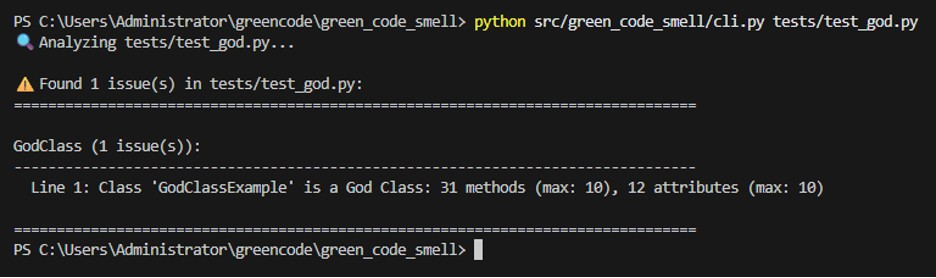
\includegraphics[width=\textwidth]{figures/chap5/godclass_before_refactor.jpg}
        \captionsetup{name=รูป}
        \caption{ก่อนการ refactor}
    \end{subfigure}
\hfill
\begin{subfigure}[t]{0.48\textwidth}
    \centering
    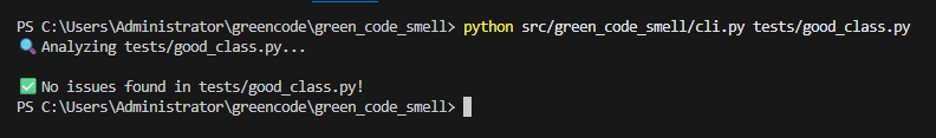
\includegraphics[width=\textwidth]{figures/chap5/godclass_after_refactor.jpg}
    \captionsetup{name=รูป}
    \caption{หลังการ refactor}
\end{subfigure}
\captionsetup{name=รูป}
\caption{ตัวอย่างผลการตรวจจับ God Class ก่อนและหลังการ refactor}
\label{fig:ch5_godclass_refactor}
\end{figure}

\begin{figure}[H]
    \centering
    \begin{subfigure}[t]{0.48\textwidth}
        \centering
        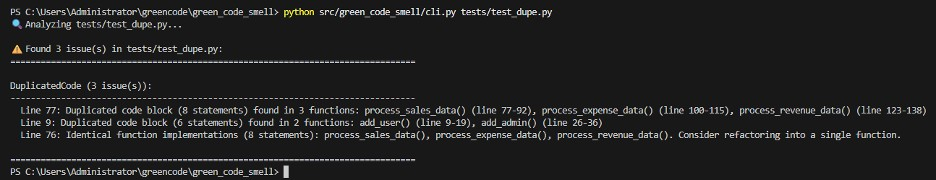
\includegraphics[width=\textwidth]{figures/chap5/duplicated_before_refactor.jpg}
        \captionsetup{name=รูป}
        \caption{ก่อนการ refactor}
    \end{subfigure}
\hfill
\begin{subfigure}[t]{0.48\textwidth}
    \centering
    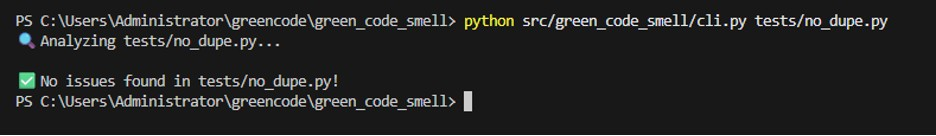
\includegraphics[width=\textwidth]{figures/chap5/duplicated_after_refactor.jpg}
    \captionsetup{name=รูป}
    \caption{หลังการ refactor}
\end{subfigure}
\captionsetup{name=รูป}
\caption{ตัวอย่างผลการตรวจจับ Duplicated Code ก่อนและหลังการ refactor}
\label{fig:ch5_duplicate_refactor}
\end{figure}

จากตัวอย่างดังกล่าวจะเห็นว่าหลังการ refactor จำนวนปัญหาที่ระบบตรวจพบลดลงอย่างชัดเจน และข้อความแสดงผลมีความตรงไปตรงมามากขึ้นต่อผู้ใช้ ช่วยให้การติดตามผลก่อนและหลังการแก้ไขสามารถทำได้ทั้งในเชิงคุณภาพและเชิงปริมาณ

% -----------------------------------------------------

\section{การประเมินผลส่วนขยาย VS Code}

การประเมินผลในระดับส่วนขยาย VS Code มีวัตถุประสงค์เพื่อทดสอบว่าระบบสามารถนำผลการวิเคราะห์จากไลบรารีมาใช้งานภายใน {\italicfont workflow} ของนักพัฒนาได้จริงหรือไม่ โดยพิจารณาทั้งด้านความถูกต้องของข้อมูลที่แสดงผล ความสะดวกในการใช้งาน และความสามารถในการนำเสนอผลวิเคราะห์ในรูปแบบที่เข้าใจง่ายสำหรับผู้ใช้ปลายทาง

\subsection{ขอบเขตการประเมินผลของ Extension}

จากโค้ดของส่วนขยาย ระบบรองรับคำสั่งหลักสำหรับการตรวจสอบ {\italicfont virtual environment} การติดตั้ง {\italicfont dependency} การวิเคราะห์ไฟล์เดี่ยว และการวิเคราะห์ทั้งโปรเจกต์ นอกจากนี้ยังสามารถเปิดผลการวิเคราะห์ผ่าน {\italicfont Webview Panel} ภายใน VS Code ได้โดยตรง

การประเมินผลของส่วนขยายจึงครอบคลุมประเด็นสำคัญดังต่อไปนี้

\begin{itemize}
    \item ความถูกต้องของการเชื่อมต่อระหว่าง Extension กับไลบรารี Python
    \item ความสามารถในการจัดการ {\italicfont environment} และ {\italicfont dependency}
    \item ความสมบูรณ์ของข้อมูลที่อ่านจาก \texttt{history.json} และผลลัพธ์จากการรันจริง
    \item ความเหมาะสมของการแสดงผลผ่าน {\italicfont Webview Dashboard}
\end{itemize}

\subsection{ผลการแสดงผลและการรายงานผลผ่าน Webview}

จาก {\italicfont implementation} ของส่วนขยาย ระบบมีการเตรียมสภาพแวดล้อม Python ผ่าน extension venv ตรวจสอบว่า CLI ของ PyGreenSense สามารถ import ได้จริง คัดลอก \texttt{history.json} ไปยัง workspace ชั่วคราวเพื่อใช้ระหว่างการรัน จากนั้นจึงเรียก PyGreenSense CLI และอ่านผลลัพธ์กลับมาทั้งจาก stdout/stderr และไฟล์ประวัติ เพื่อส่งต่อไปยังผลลัพธ์ใน webview panel

ในระดับการแสดงผล ส่วนขยายสามารถสรุปข้อมูลการวิเคราะห์ออกมาในรูปของ {\italicfont metric cards} และรายละเอียดเชิงลึก เช่น ปริมาณคาร์บอนที่ปล่อย จำนวนปัญหาที่ตรวจพบ ค่า CFP, LOC, ระยะเวลาในการประมวลผล พลังงานที่ใช้ อัตราการปล่อยคาร์บอน ภูมิภาคของ {\italicfont grid} ค่า SCI ต่อบรรทัด และค่า SCI ต่อ CFP ได้ นอกจากนี้ ระบบยังรองรับการแสดงผลประวัติการวิเคราะห์ ({\italicfont history view}) และ {\italicfont program output} จากการรันล่าสุด

รูป \ref{fig:ch5_webview_analysis} ถึงรูป \ref{fig:ch5_webview_output} แสดงหน้าจอการทำงานจริงของ {\italicfont Webview Dashboard} โดยครอบคลุมทั้งแท็บ Analysis, Issues, History และ Output ตามลำดับ ซึ่งช่วยยืนยันว่าระบบสามารถรวมข้อมูลสรุป การแสดงปัญหารายบรรทัด ประวัติการรัน และผลจาก program output ไว้ในพื้นที่รายงานเดียวได้อย่างครบถ้วน

\begin{figure}[H]
    \centering
    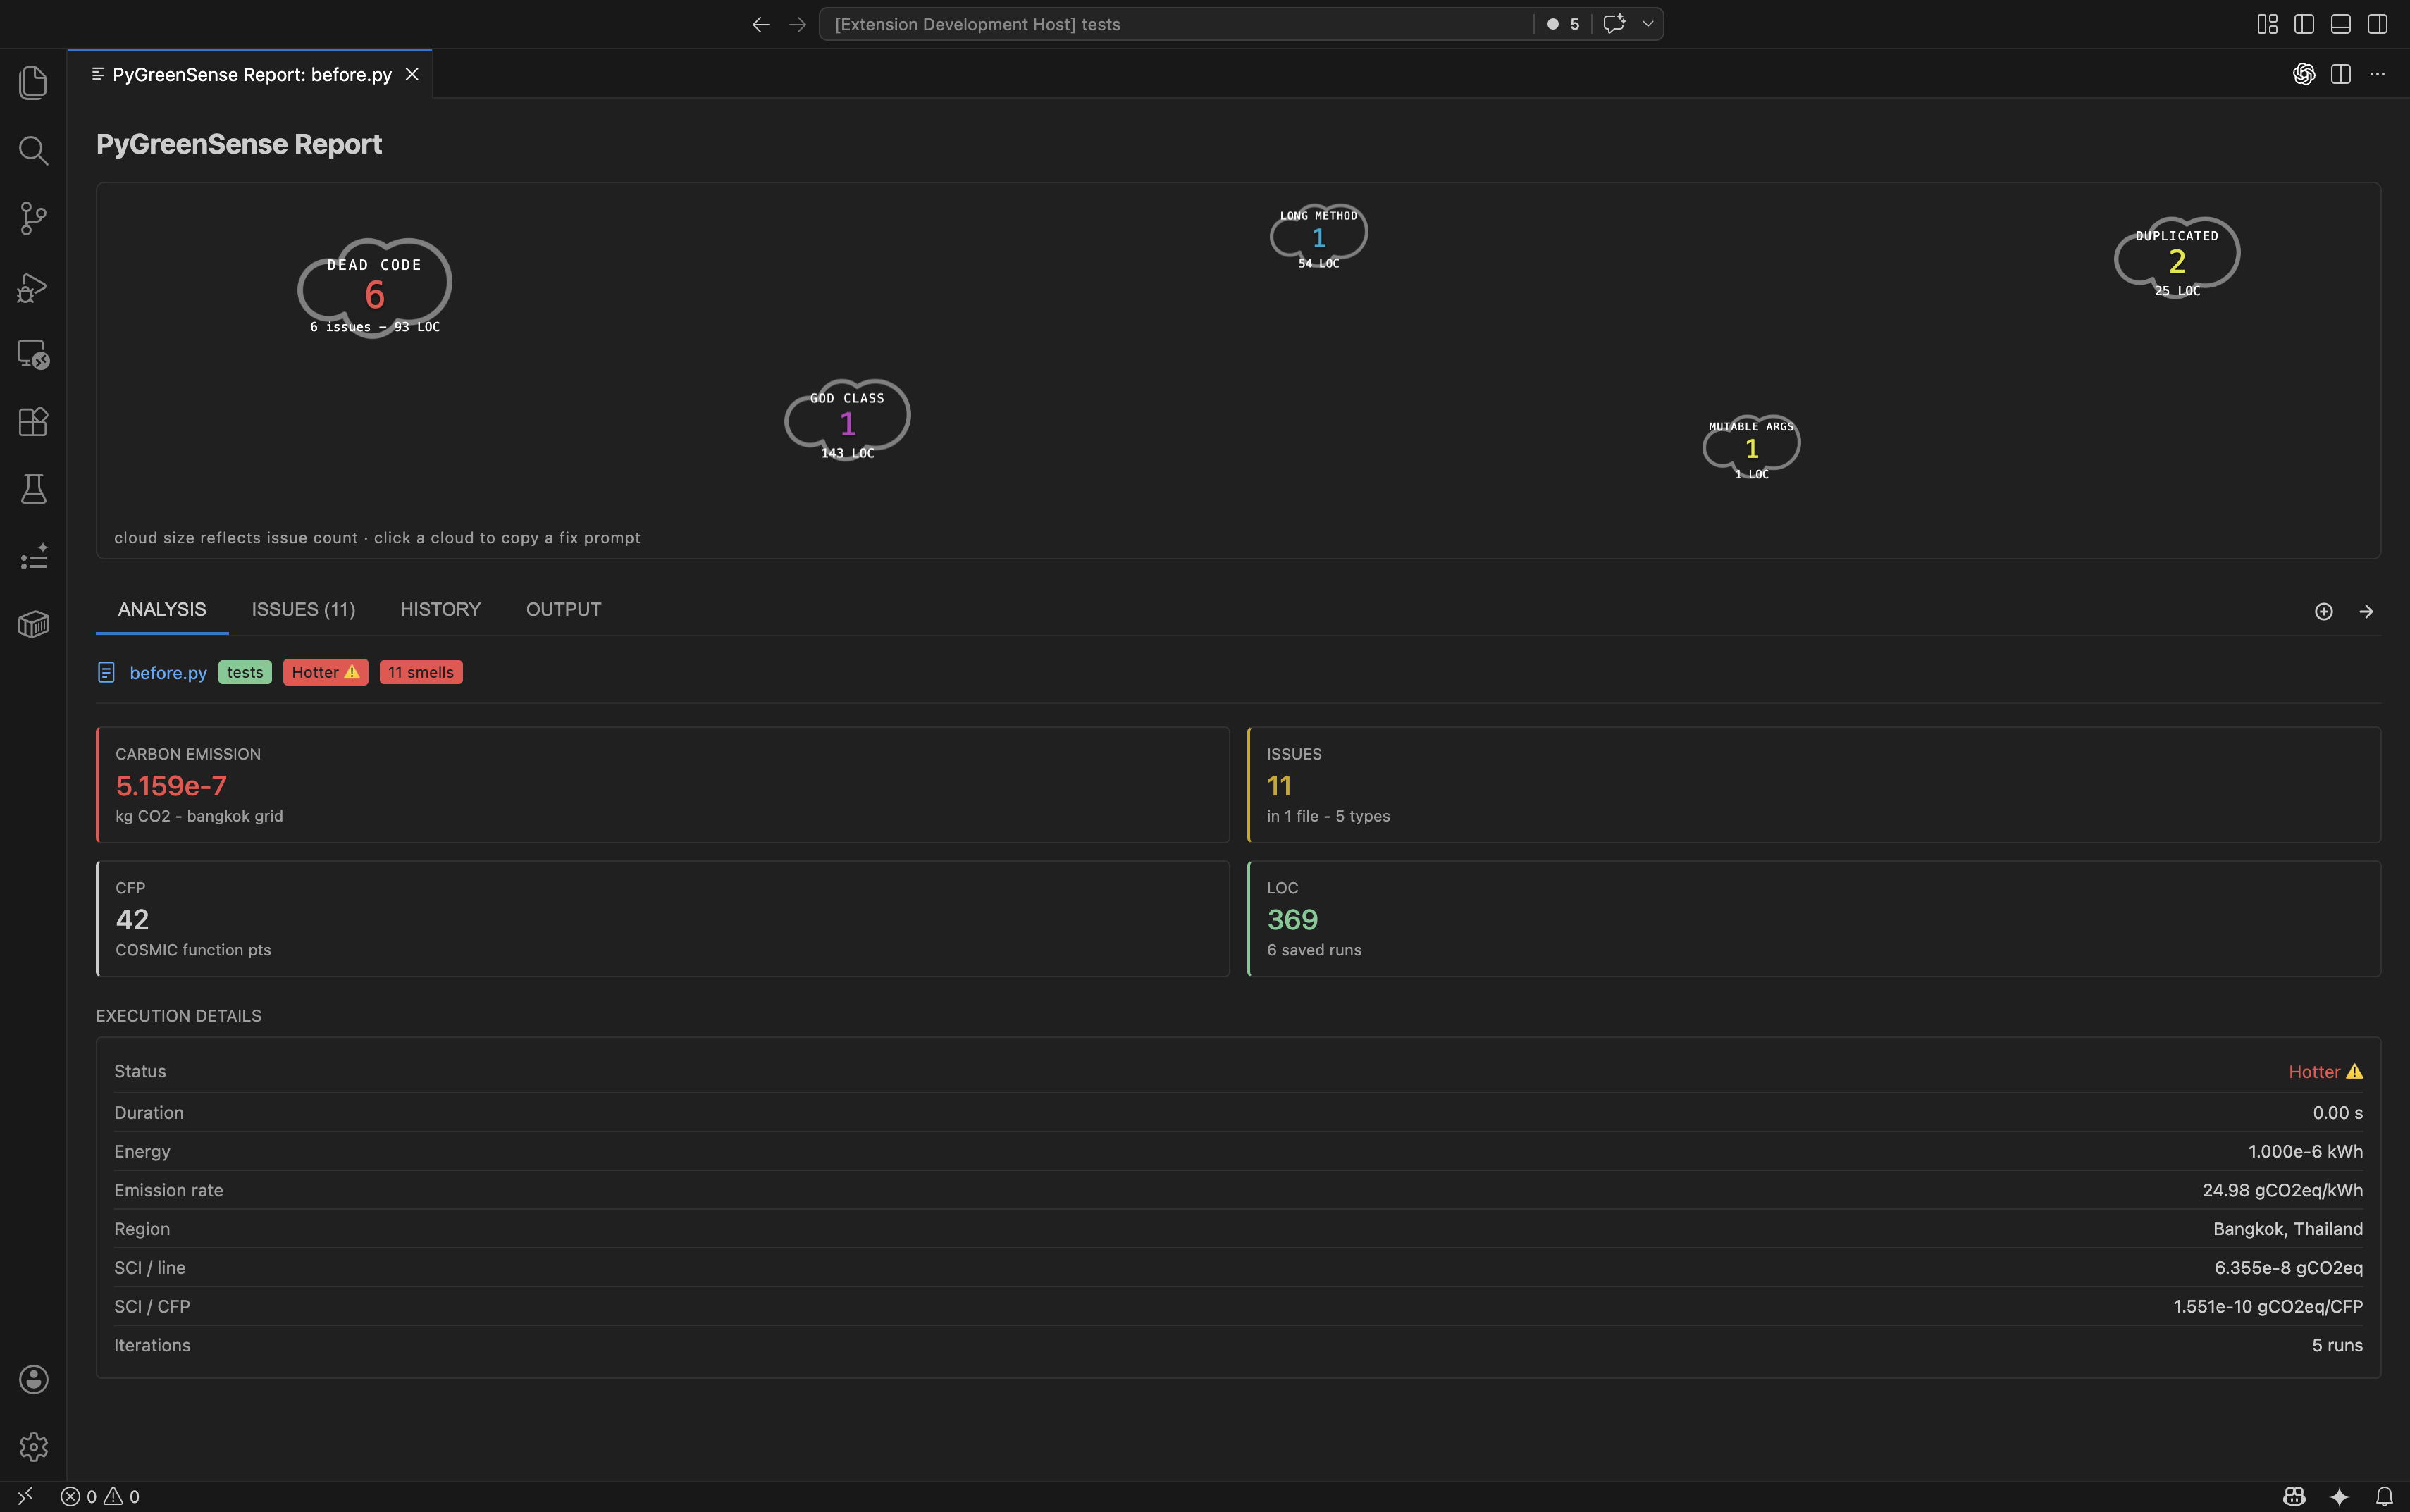
\includegraphics[width=\textwidth]{figures/chap5/webview_analysis_tab.png}
    \captionsetup{name=รูป}
    \caption{หน้าจอแท็บ Analysis ของ Webview Dashboard}
    \label{fig:ch5_webview_analysis}
\end{figure}

\begin{figure}[H]
    \centering
    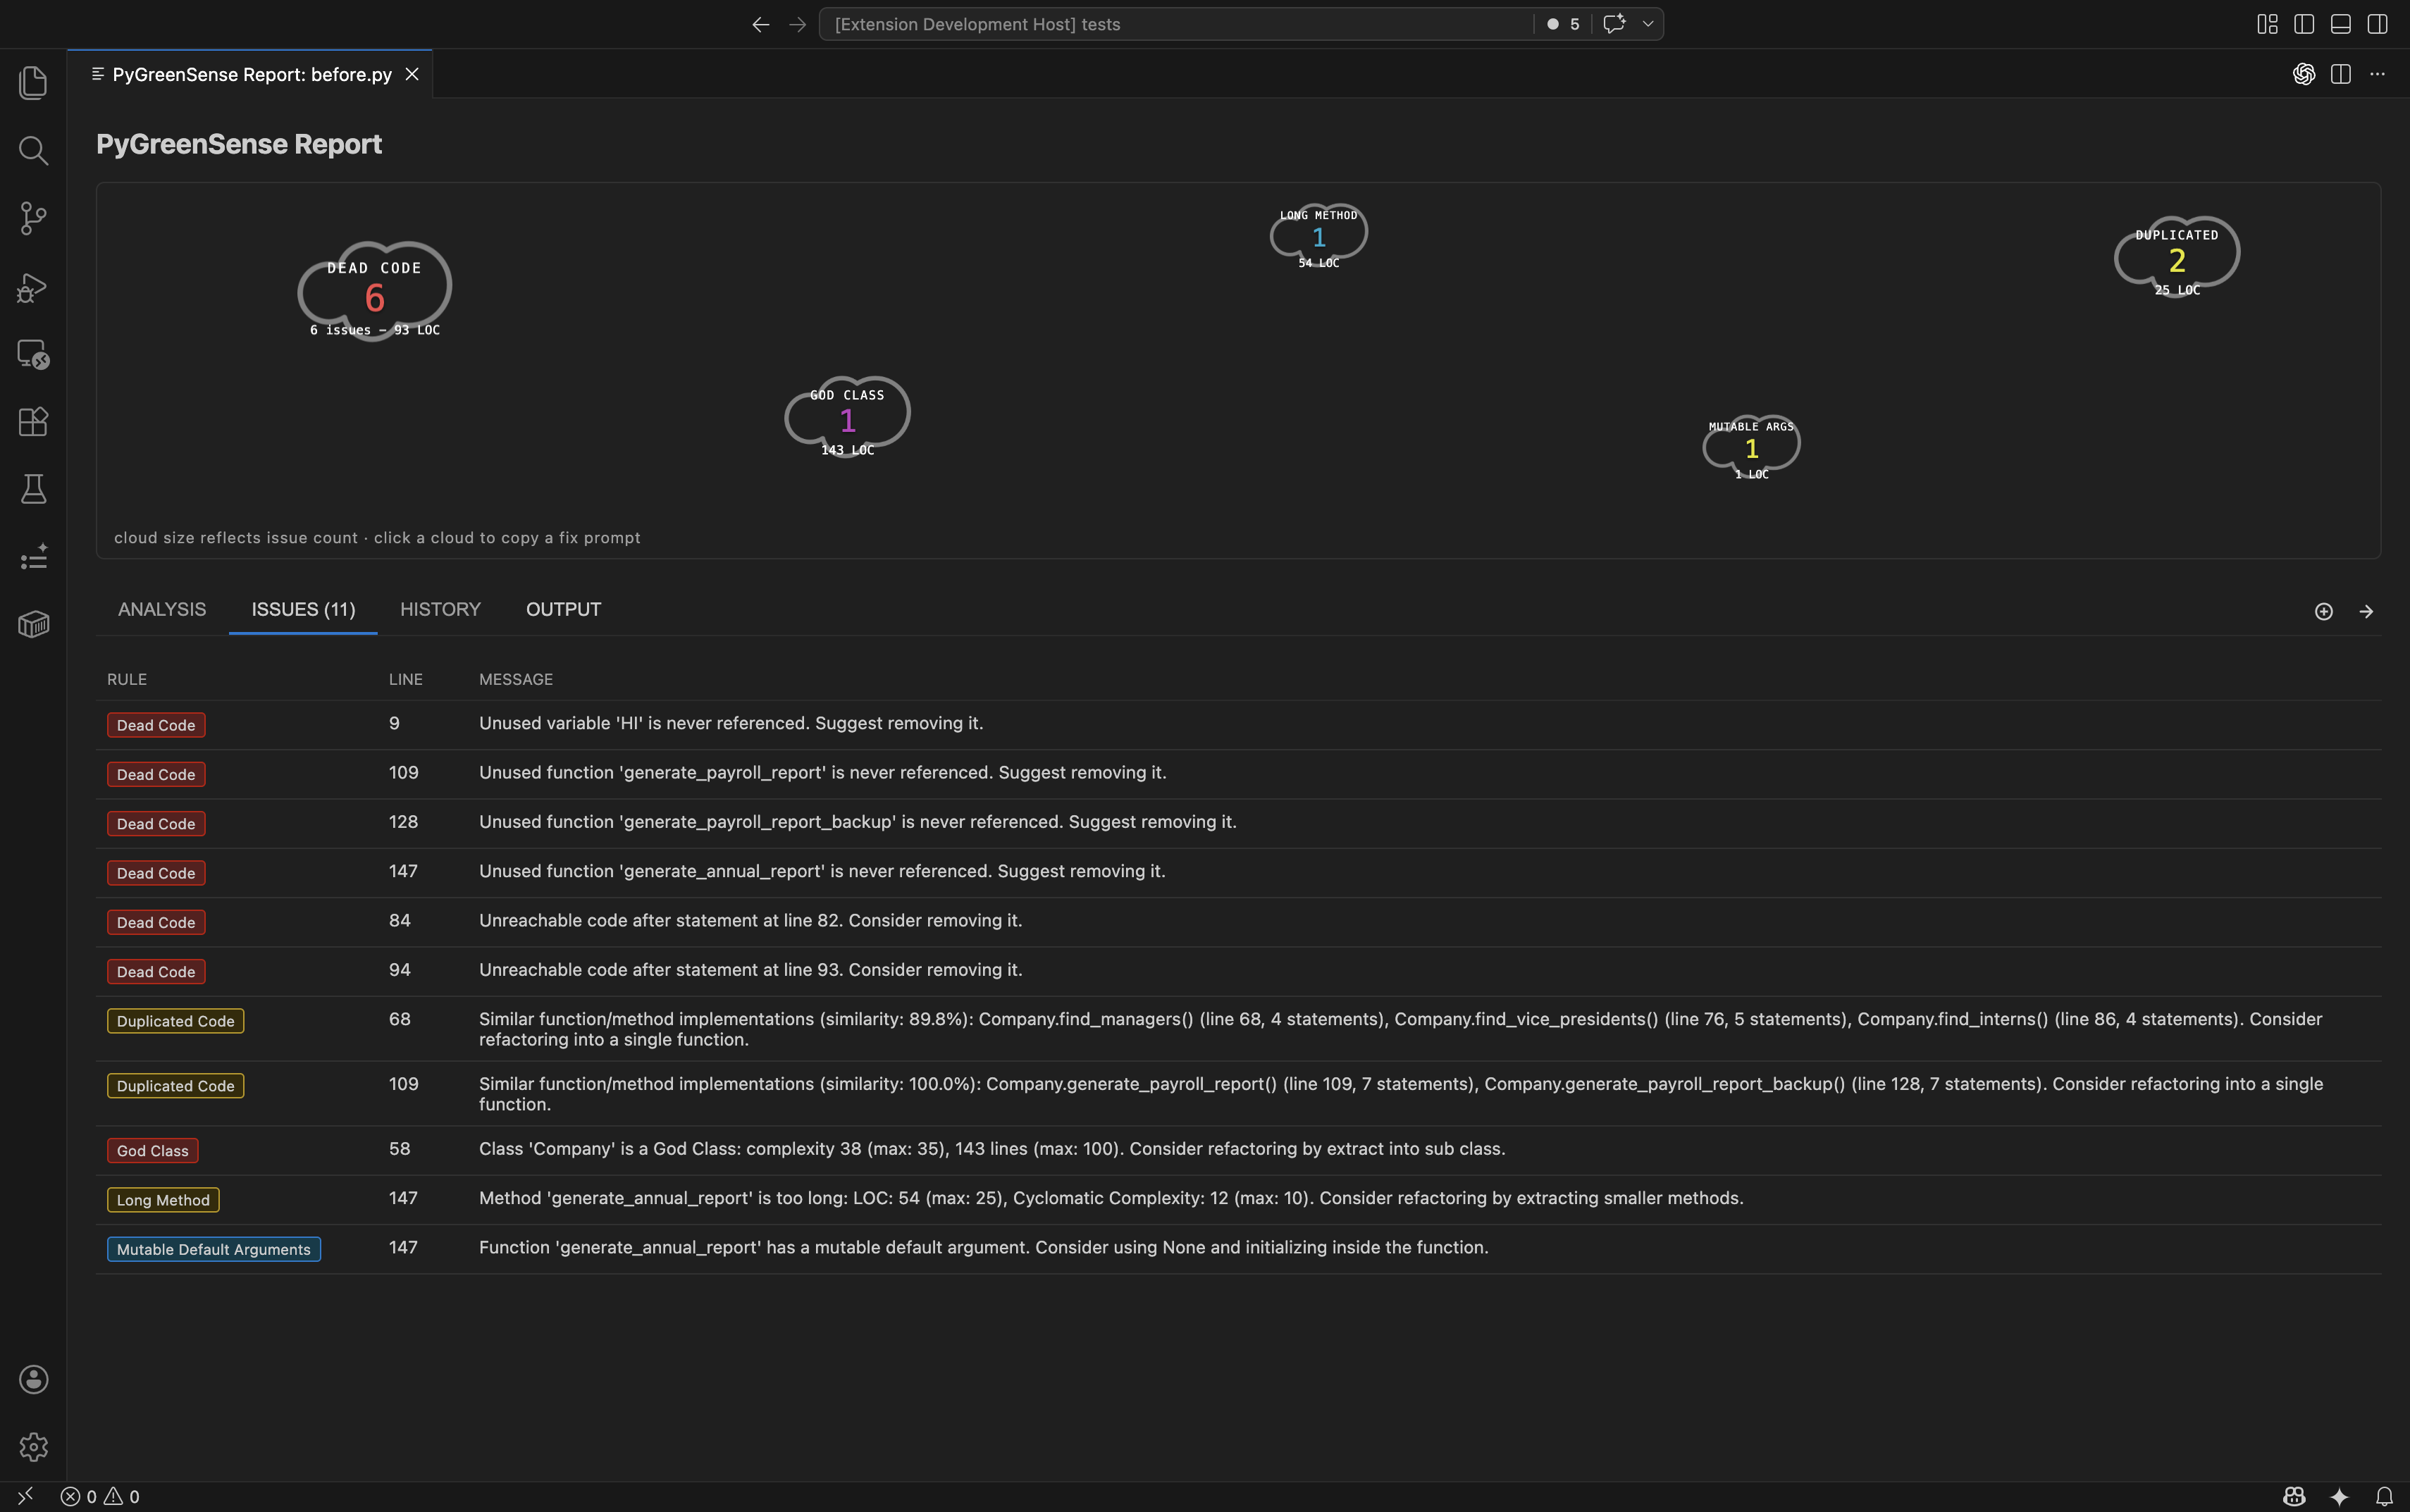
\includegraphics[width=\textwidth]{figures/chap5/webview_issues_tab.png}
    \captionsetup{name=รูป}
    \caption{หน้าจอแท็บ Issues ของ Webview Dashboard}
    \label{fig:ch5_webview_issues}
\end{figure}

\begin{figure}[H]
    \centering
    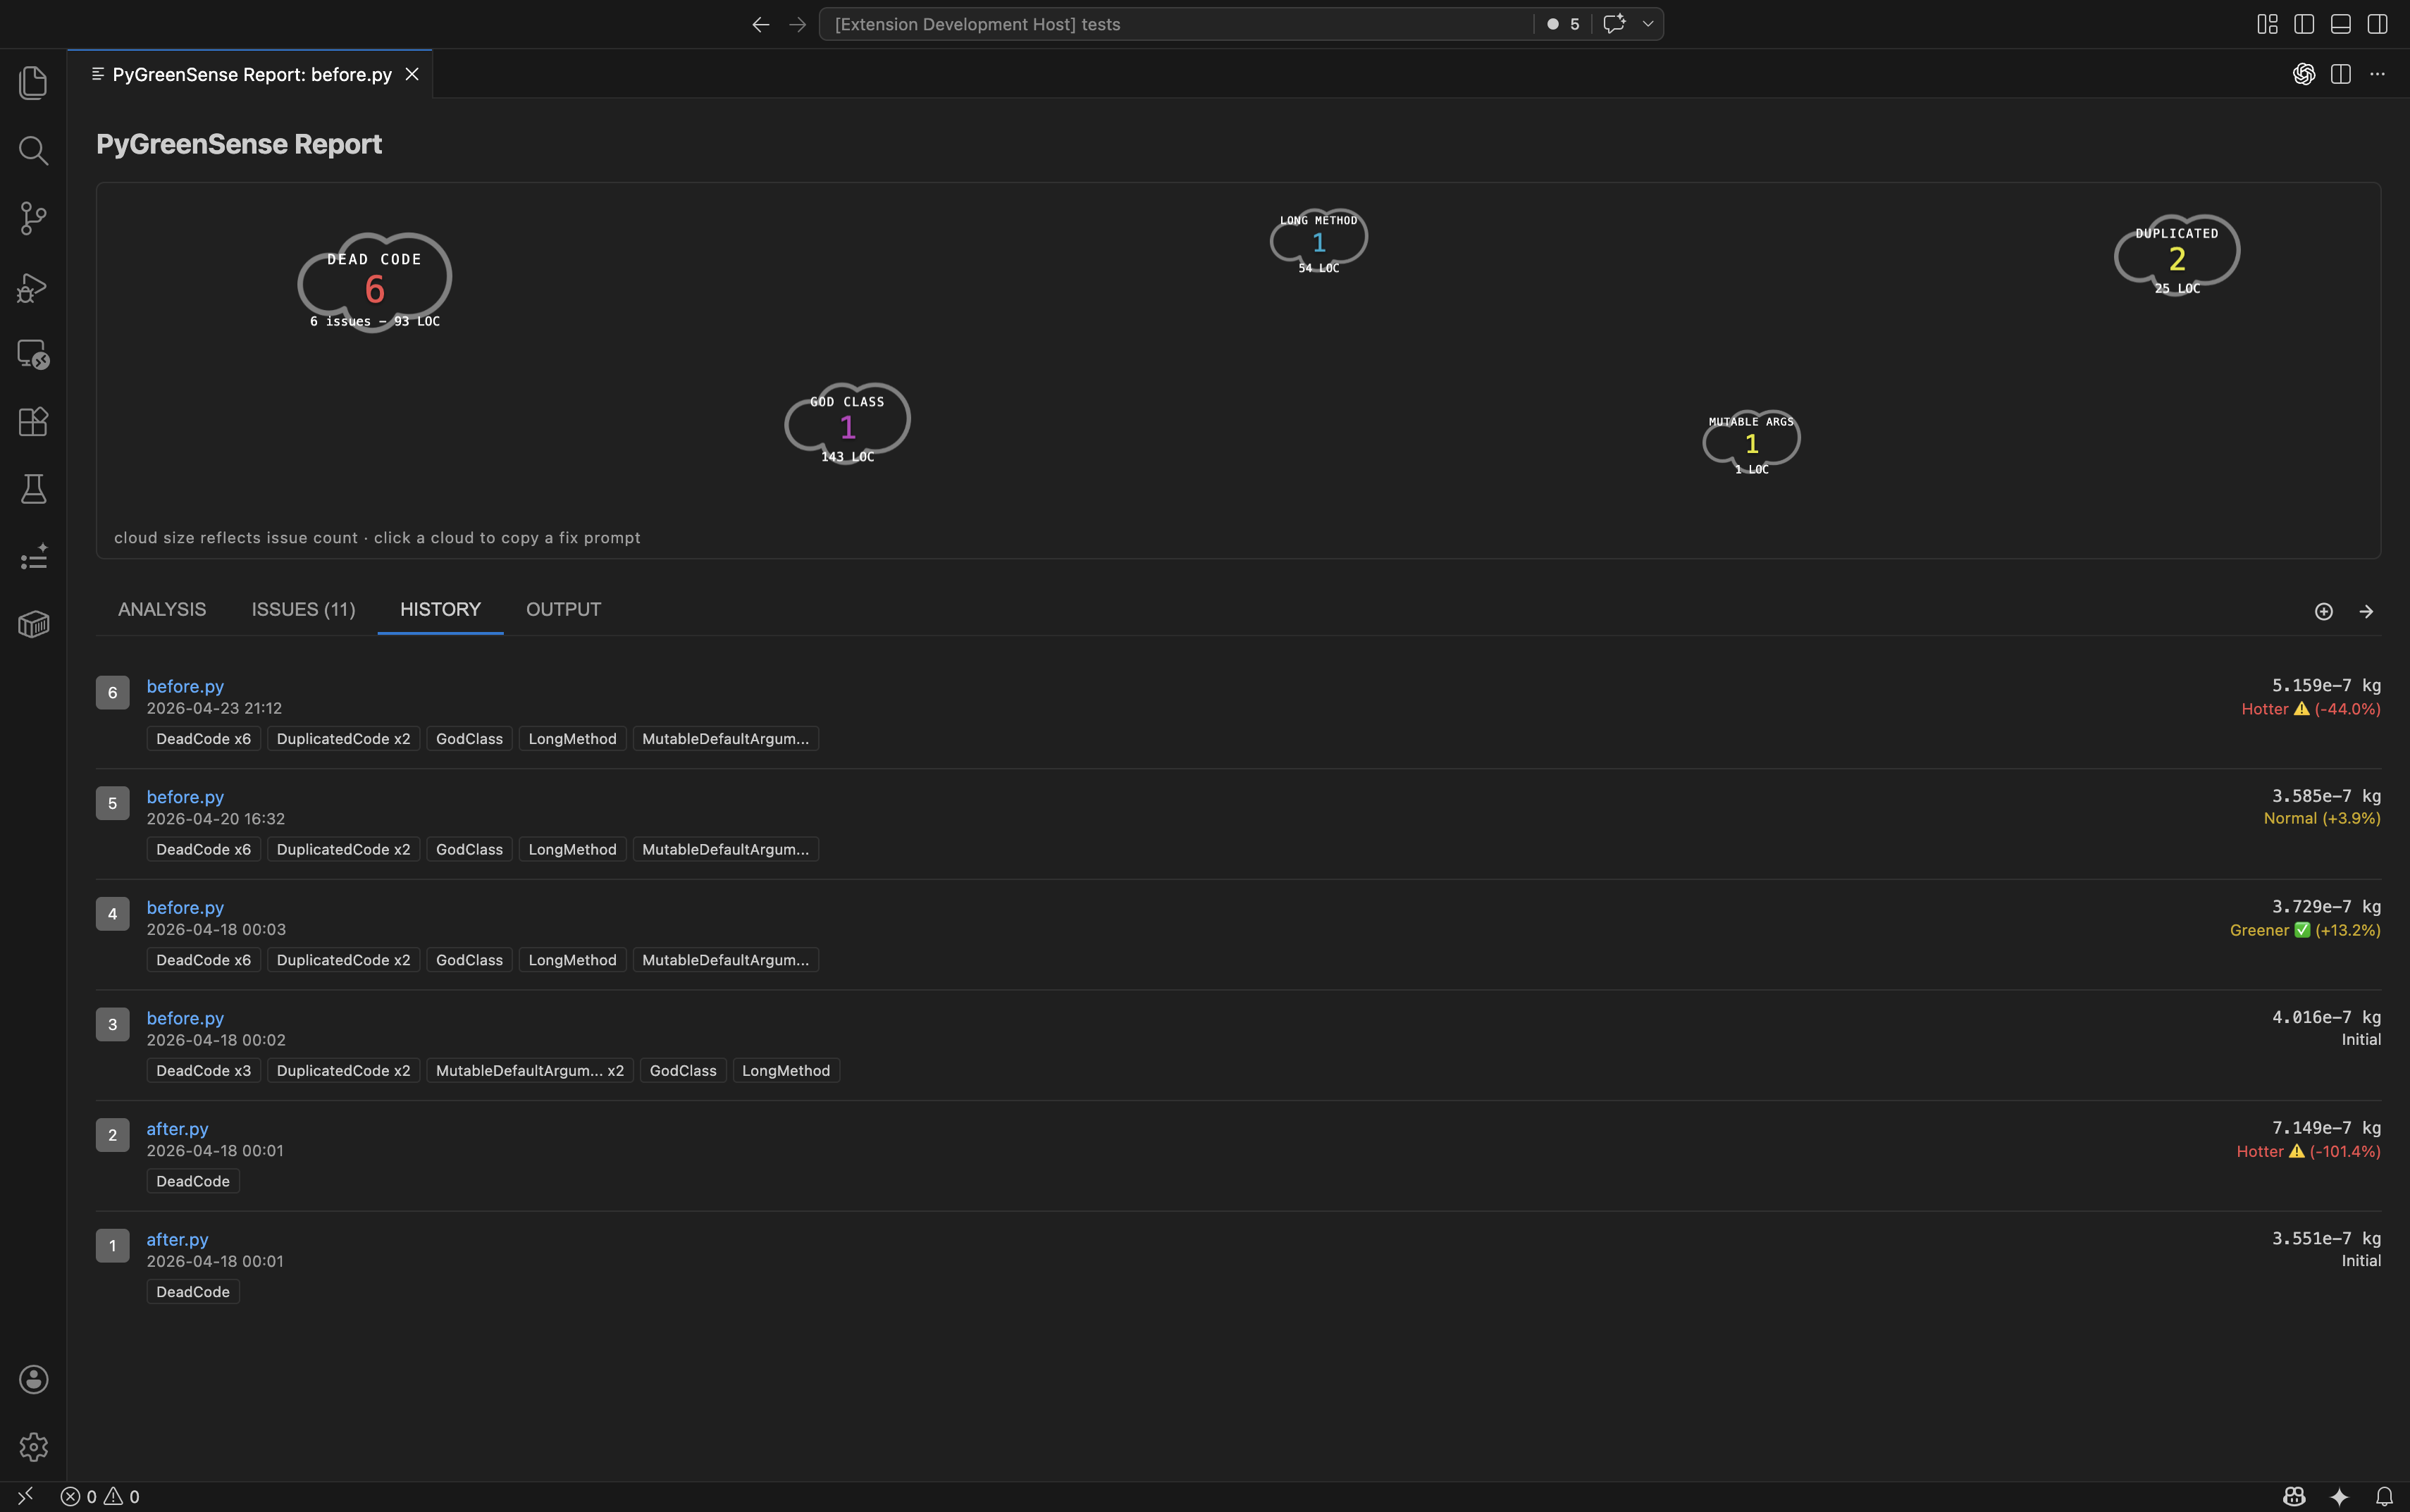
\includegraphics[width=\textwidth]{figures/chap5/webview_history_tab.png}
    \captionsetup{name=รูป}
    \caption{หน้าจอแท็บ History ของ Webview Dashboard}
    \label{fig:ch5_webview_history}
\end{figure}

\begin{figure}[H]
    \centering
    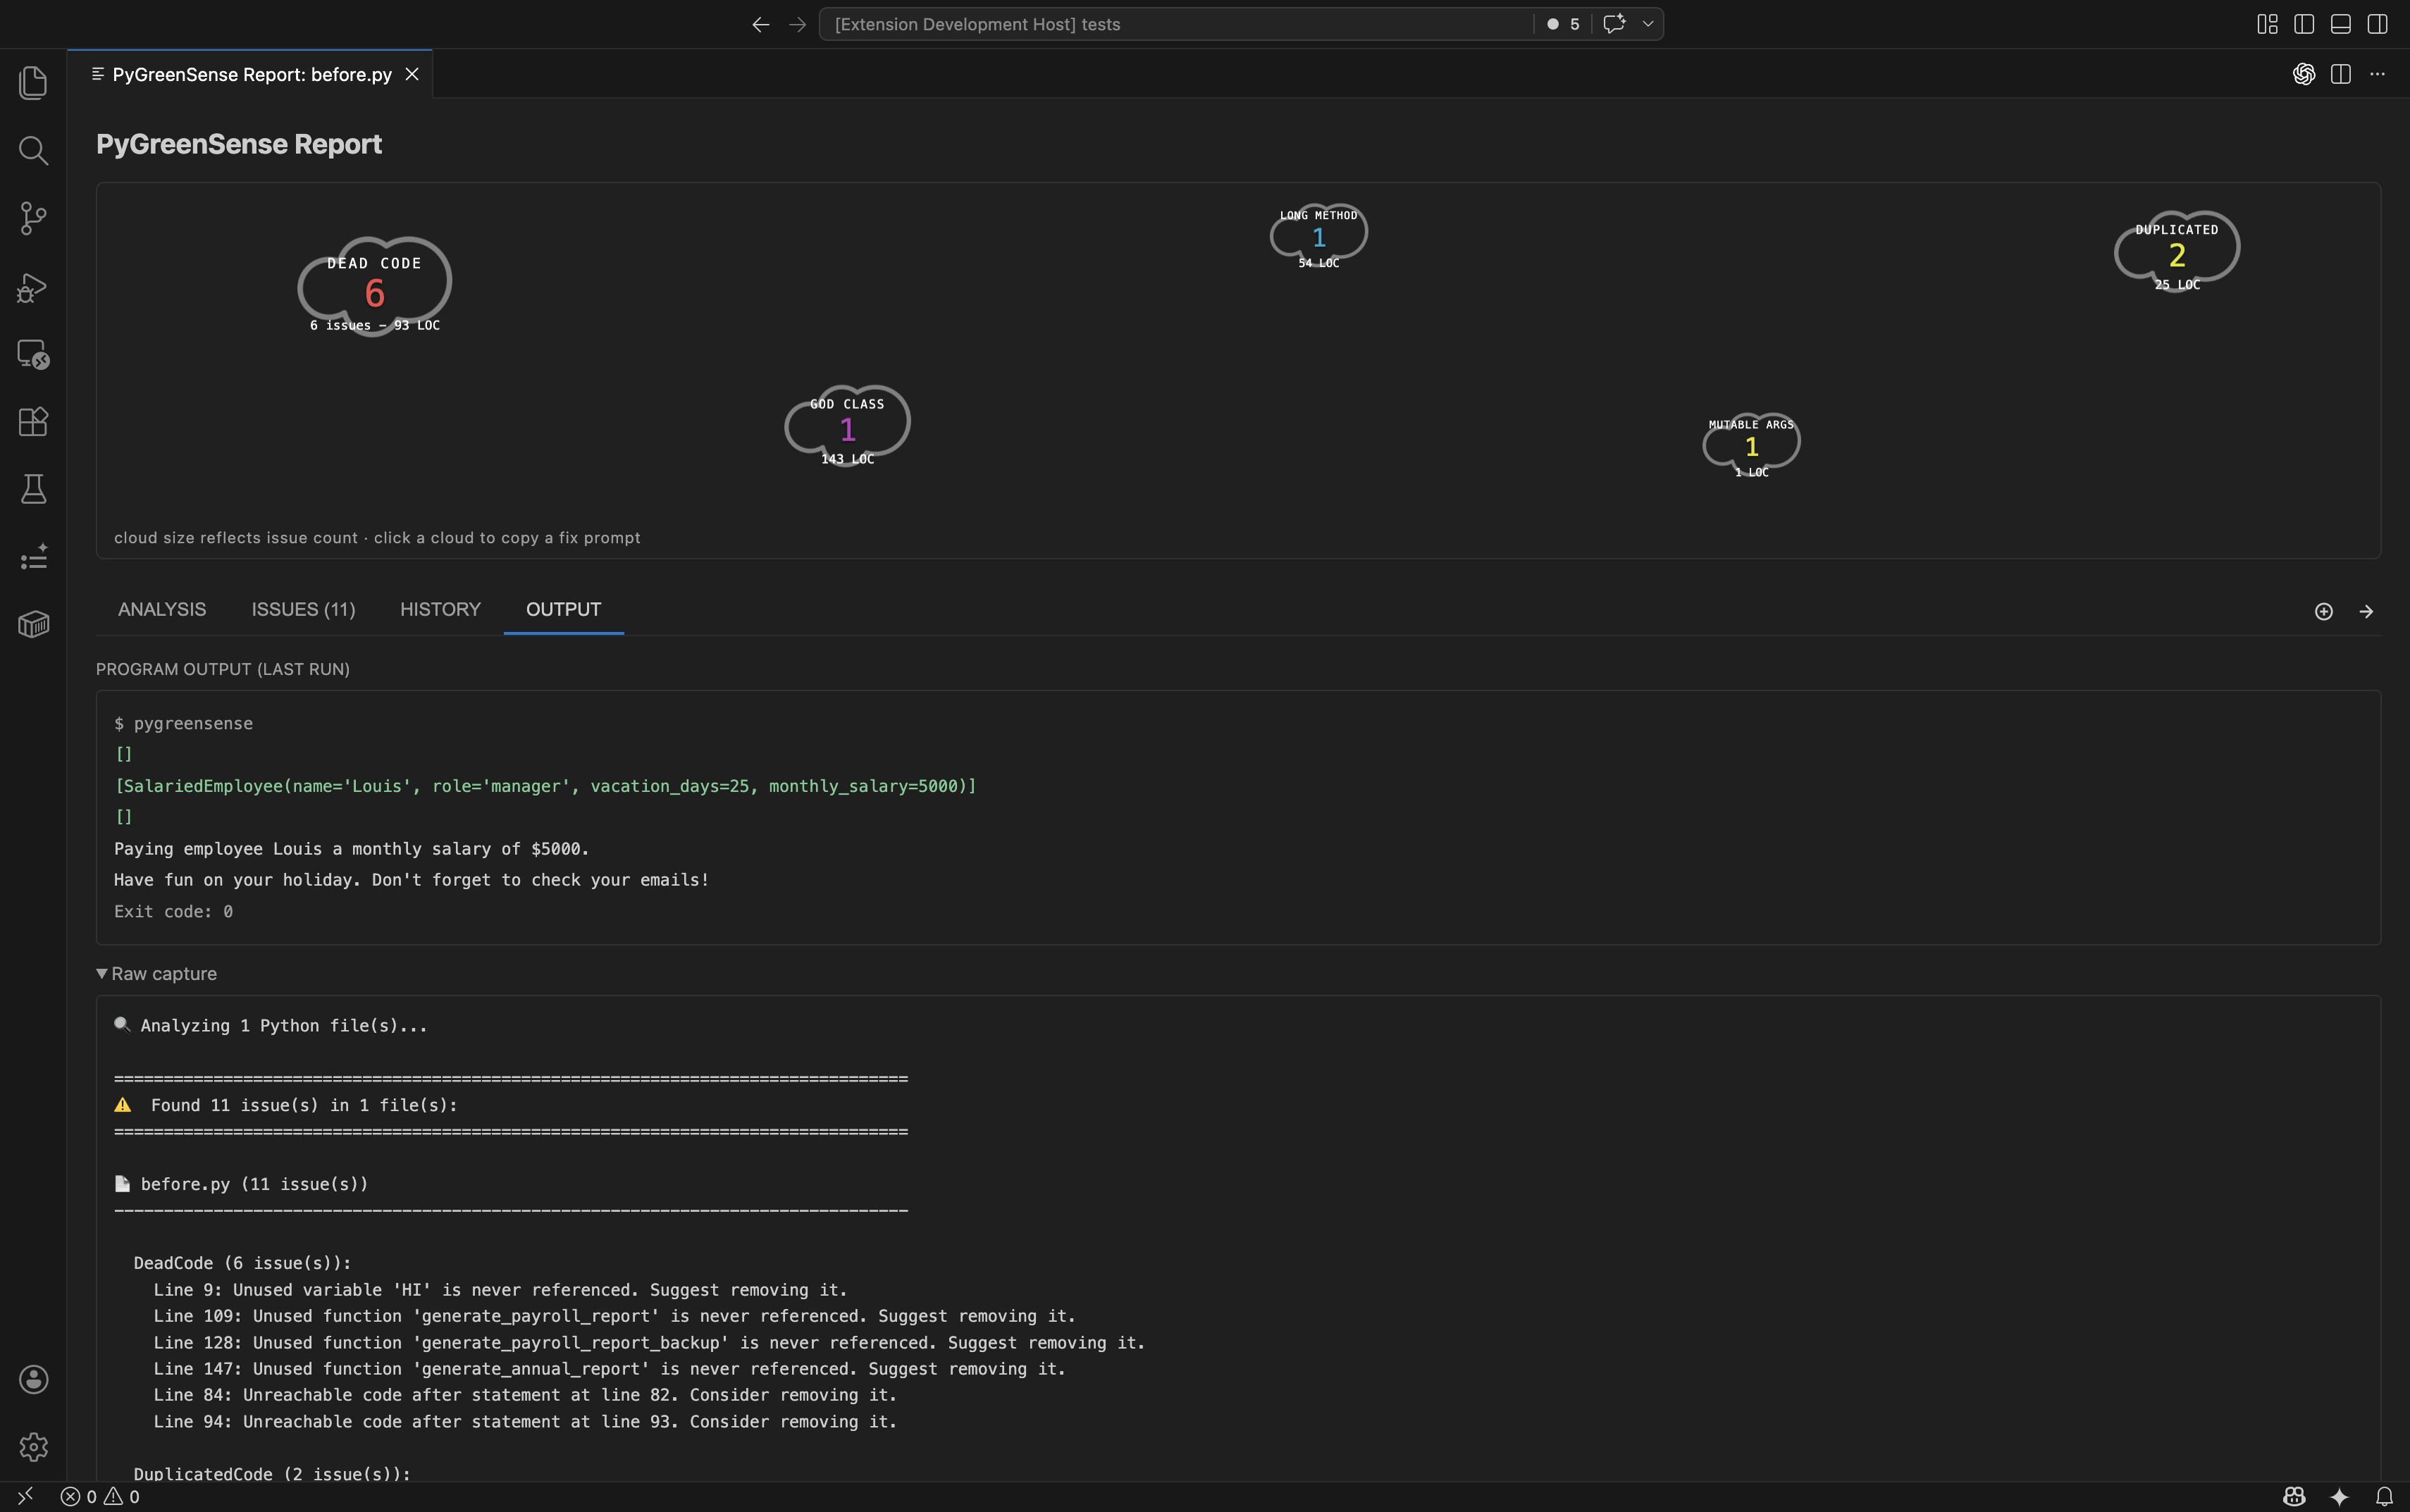
\includegraphics[width=\textwidth]{figures/chap5/webview_output_tab.png}
    \captionsetup{name=รูป}
    \caption{หน้าจอแท็บ Output ของ Webview Dashboard}
    \label{fig:ch5_webview_output}
\end{figure}

\subsection{การประเมินผลมาตรวัดด้านพลังงานและคาร์บอน}

ในระดับการแสดงผล ส่วนขยายรองรับการนำเสนอข้อมูลที่สอดคล้องกับแนวคิดด้าน {\italicfont Software Carbon Intensity (SCI)} และการวัดผลผ่าน {\italicfont CodeCarbon} โดยระบบมีช่องแสดงค่า {\italicfont SCI / line} และ {\italicfont SCI / CFP} อย่างชัดเจน รวมถึงรองรับการแสดงค่า CFP และปริมาณการปล่อยคาร์บอนจากการวิเคราะห์ในแต่ละรอบ

ในเชิงวิธีวิทยา การมีมาตรวัดดังกล่าวช่วยให้ผู้ใช้ไม่ได้เห็นเพียงจำนวน {\italicfont code smell} เท่านั้น แต่ยังเห็นผลกระทบด้านพลังงานและสิ่งแวดล้อมในรูปแบบที่สามารถตีความเชิงเปรียบเทียบได้ ซึ่งสอดคล้องกับแนวคิด {\italicfont SCI per functional unit} ที่กล่าวไว้ในบททฤษฎีที่เกี่ยวข้อง \cite{sciSpecification,codecarbonMethodology,abran2018cosmic}

ดังแสดงในรูป \ref{fig:ch5_webview_analysis} ส่วนของ metric cards และ execution details ถูกออกแบบให้ผู้ใช้เห็นค่าหลัก เช่น carbon emission, CFP, LOC, SCI / line และ SCI / CFP พร้อมกันในหน้ารายงานเดียว ทำให้การตีความผลในเชิงก่อน/หลังการปรับปรุงโค้ดสามารถทำได้สะดวกขึ้น ขณะเดียวกันรูป \ref{fig:ch5_webview_history} และรูป \ref{fig:ch5_webview_output} ช่วยยืนยันว่าระบบรองรับการติดตามผลย้อนหลังและตรวจสอบผลจากการรันล่าสุดได้ภายในรายงานเดียวกัน

\subsection{การประเมินจากการใช้งานจริงของผู้ใช้}

ในส่วนนี้ใช้สำหรับการวัดผลจากการใช้งานจริงของผู้ใช้ เช่น ความพึงพอใจต่อความชัดเจนของ webview ความสะดวกในการใช้งานคำสั่ง ความเข้าใจในค่าพลังงานและคาร์บอน หรือความสามารถของระบบในการช่วยให้ผู้ใช้ตัดสินใจปรับปรุงโค้ดได้ดีขึ้น

อย่างไรก็ตาม ในขอบเขตของฉบับปัจจุบันยังไม่ได้มีการเก็บข้อมูลเชิงปริมาณจากผู้ใช้จริงอย่างเป็นระบบ เช่น แบบสอบถามหรือการทดลองเชิง usability study ดังนั้นบทนี้จึงรายงานผลการประเมินเชิงฟังก์ชันของระบบเป็นหลัก ขณะที่การประเมินความพึงพอใจ ความเข้าใจต่อ metric และผลต่อการตัดสินใจ refactor ของผู้ใช้ จะถูกเสนอเป็นแนวทางการศึกษาต่อยอดในอนาคต

\subsection{การวิเคราะห์ผลในระดับ Extension}

ผลการประเมินในระดับส่วนขยายสะท้อนให้เห็นว่า {\italicfont PyGreenSense Extension} สามารถนำข้อมูลที่ได้จากไลบรารีมาแปลงเป็นรายงานที่มีความเป็นมิตรต่อผู้ใช้และเหมาะกับการใช้งานในสภาพแวดล้อมการพัฒนาจริง โดยเฉพาะการรวมข้อมูลด้าน {\italicfont code smell}, {\italicfont carbon emission}, CFP และประวัติการวิเคราะห์ไว้ในหน้ารายงานเดียว ทำให้ผู้ใช้สามารถมองเห็นทั้งภาพรวมและรายละเอียดของปัญหาได้พร้อมกัน

% -----------------------------------------------------

\section{สรุปผลการประเมิน}

จากการประเมินผลทั้งในระดับไลบรารีและส่วนขยาย VS Code สามารถสรุปได้ว่า {\italicfont PyGreenSense} มีศักยภาพในการทำหน้าที่เป็นเครื่องมือสำหรับตรวจจับ {\italicfont Green Code Smell} ในภาษา Python และสนับสนุนการประเมินผลกระทบด้านพลังงานและคาร์บอนใน {\italicfont workflow} ของนักพัฒนาได้อย่างเป็นรูปธรรม โดยในระดับไลบรารี ระบบสามารถเปรียบเทียบกับเครื่องมืออ้างอิงในอุตสาหกรรมได้ ขณะที่ในระดับ Extension ระบบสามารถนำเสนอผลลัพธ์ผ่าน {\italicfont Webview Dashboard} พร้อมข้อมูลประวัติและมาตรวัดเชิงพลังงานที่เกี่ยวข้องได้อย่างครบถ้วน

อย่างไรก็ตาม หากต้องการให้การประเมินผลมีความสมบูรณ์ยิ่งขึ้นในฉบับสุดท้าย ควรเพิ่มเติมตารางผลการทดลองจริง ค่าความแม่นยำหรือความสอดคล้องเชิงปริมาณของแต่ละ {\italicfont rule} ตัวอย่างผลการเปรียบเทียบก่อนและหลังการปรับปรุงโค้ด และผลจากการใช้งานจริงของผู้ใช้ เพื่อให้การอภิปรายผลมีความชัดเจนและตรวจสอบย้อนกลับได้มากขึ้น
